\subsection{AI Generation Pipelines}
\label{sec:impl_ai_pipelines}

The quiz and interview generation pipelines share a common architectural pattern: a multi-stage orchestrator that threads a single \texttt{pipeline\_run\_id} through every LLM call so all \texttt{ai\_model\_calls} audit rows roll up to one \texttt{ai\_pipeline\_runs} parent. Each stage is a pure function that receives its inputs and returns typed outputs, making stages independently testable and replaceable.

\subsubsection{Hybrid Retrieval}
\label{sec:impl_retrieval}

Both pipelines begin with a hybrid retrieval stage that combines dense vector search with sparse BM25 full-text search, then fuses the two ranked lists using Reciprocal Rank Fusion (RRF).

\paragraph{Dense retrieval}
The \texttt{pgvector} retrieval module (\path{ai/retrieval/pgvector.py}) performs an approximate nearest-neighbour search using the \texttt{<=>} cosine distance operator on the \texttt{halfvec(3072)} embedding column. The query text is embedded with the same model used during ingestion, and the top-$k$ chunks are returned ordered by ascending cosine distance.

\paragraph{Sparse retrieval}
The BM25 module (\path{ai/retrieval/bm25.py}) queries the \texttt{content\_tsv} column using PostgreSQL's \texttt{ts\_rank\_cd} function. This captures exact keyword matches that may be missed by the semantic search, particularly for technical terms, acronyms, and proper nouns.

\paragraph{RRF fusion}
The two ranked lists are fused in \path{ai/retrieval/fusion.py} using the weighted RRF formula adapted from the Anthropic Contextual Retrieval cookbook~\cite{anthropic2024contextual}:

\begin{equation}
    \text{score}(c) = w_{\text{sem}} \cdot \frac{1}{\text{rank}_{\text{sem}}(c) + 1} + w_{\text{bm25}} \cdot \frac{1}{\text{rank}_{\text{bm25}}(c) + 1}
\end{equation}

where $w_{\text{sem}} = 0.8$ and $w_{\text{bm25}} = 0.2$ by default (configurable via \texttt{hybrid\_semantic\_weight} and \texttt{hybrid\_bm25\_weight} settings). Chunks absent from one list contribute zero from that leg. The fused list is re-ranked by descending score and the top-$N$ chunks are forwarded to the generation stage.

\paragraph{Role-based filtering}
A \texttt{RoleFilter} post-processor restricts retrieved chunks to those the requesting user is authorised to access, based on their course enrollment and organisation membership. This ensures that quiz questions are generated only from materials the student has been granted access to.

\paragraph{MMR re-ranking (optional)}
When \texttt{mmr\_enabled} is true, Maximal Marginal Relevance~\cite{carbonell1998mmr} is applied after fusion to reduce redundancy in the retrieved set. MMR iteratively selects the chunk that maximises relevance to the query while minimising similarity to already-selected chunks, producing a more diverse context window for the LLM.

\subsubsection{Quiz Generation Pipeline}
\label{sec:impl_quiz_pipeline}

The full quiz generation pipeline (\path{features/quizzes/ai/pipelines/full.py}) executes six stages in sequence. Figure~\ref{fig:quiz_generation_flow} in Appendix~\ref{appendix:algorithm} places these stages in the wider request they serve --- the synchronous dispatch that returns before any of them run, the durable run row they report against, and the poll by which the teacher's browser learns the outcome.

\begin{enumerate}
    \item \textbf{Retrieval} — hybrid retrieval as described above, returning the top-$N$ fused chunks plus optional knowledge graph context.
    \item \textbf{Ideation} — an LLM call that, given the retrieved chunks and a course outline, produces a list of question \emph{topics} (ideation targets). The outline is either provided by the caller or synthesised from the chunk metadata. The ideation stage oversamples by a factor of 1.5 to give the downstream validation stage room to reject low-quality drafts.
    \item \textbf{Generation} — for each ideation target, an LLM call generates a multiple-choice question with four options, a correct answer key, and an explanation. Prompts are rendered from Jinja2 templates in \path{ai/stages/generation/prompts/}.
    \item \textbf{Validation} — each generated question is passed to a second LLM call that checks factual accuracy, option quality, and alignment with the source chunks. The validator returns a verdict (\texttt{accept}, \texttt{revise}, or \texttt{reject}) with a rationale. Rejected questions are discarded; revised questions are patched in place.
    \item \textbf{Deduplication} — accepted questions are compared pairwise using embedding cosine similarity. Questions whose embeddings exceed a configurable similarity threshold are deduplicated, keeping the higher-quality variant.
    \item \textbf{Persistence} — accepted, deduplicated questions are written to the \texttt{quiz\_questions} and \texttt{quiz\_question\_options} tables as a draft batch, associated with the quiz and the \texttt{pipeline\_run\_id}.
\end{enumerate}

\subsubsection{Interview Question Generation}

\begin{figure}[H]
    \centering
    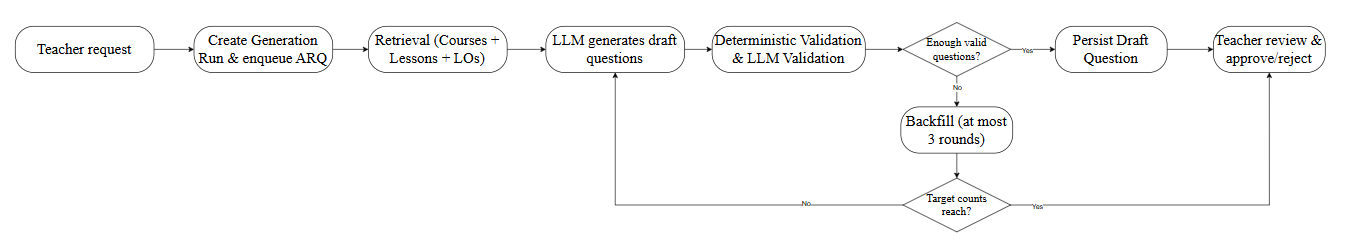
\includegraphics[width=0.95\textwidth]{graphics/act-diagrams/act_interview_generation.png}
    \caption{Interview Question Generation Pipeline.}
    \label{fig:interview_question_generation}
\end{figure}

As shown in Figure~\ref{fig:interview_question_generation}, the pipeline retrieves authorised course material and learning outcomes, then creates draft open-ended questions with suggested assessment guidance. Basic validation checks grounding and outcome alignment before accepted drafts are stored for teacher review. Only teacher-approved questions enter a published interview configuration.

\subsubsection{LLM Gateway and Audit}
\label{sec:impl_llm_gateway}

All LLM calls are routed through \texttt{LLMGateway} (\path{ai/llm/gateway.py}), which provides a uniform interface over any OpenAI-compatible endpoint. The gateway:
\begin{itemize}
    \item Selects the model and API key based on the \texttt{LLMRole} (e.g., \texttt{QUIZ\_GENERATION}, \texttt{EMBEDDING}, \texttt{KG\_BUILD}), allowing different roles to use different models or providers.
    \item Parses LLM responses robustly: it first attempts strict \texttt{json.loads}, then extracts from a fenced code block, then uses \texttt{raw\_decode} to tolerate trailing commentary from models that ignore the \texttt{json\_object} response format.
    \item Writes one \texttt{ai\_model\_calls} row per call recording the model name, prompt and completion token counts, computed cost (via a per-model pricing table), latency, and the \texttt{pipeline\_run\_id} grouping key.
\end{itemize}

\paragraph{Nothing generated reaches a learner unreviewed}
The stages above end at the gateway, but the pipeline does not end at the model. Every artefact a generation run produces --- quiz questions, interview questions, extracted knowledge --- is written in a pending state and requires a human decision before it becomes visible to a student. A teacher approves it, edits it, or rejects it; the original and the edited form are both retained, so the quality of the generation itself stays measurable over time rather than being overwritten by the corrections applied to it.

This gate is the reason the retrieval work above is worth doing rather than merely interesting. Retrieval quality determines how much of the teacher's attention each generated item consumes: grounded, deduplicated, access-filtered context produces drafts that are mostly approved as they stand, whereas poor retrieval produces drafts that are individually plausible and collectively wrong, which costs more to review than to write. The pipeline is therefore tuned for reviewer throughput, not for autonomy --- the system never proposes to publish its own output.
